\documentclass{article}

% \usepackage{geometry}
\usepackage{graphicx}
\usepackage{amsmath}
\usepackage{hyperref}

\title{PA1: Stacks}
\author{Kevin Lei}
\date{February 6, 2024}

\begin{document}

\maketitle

\section{Introduction}

\indent This programming assignment focuses on three different implementations of the stack data structure. 
The stack consists of an ordered collection of items where the addition and removal of items is done at the same end.
Since the stack is just an abstract data type, we have multiple ways to implement it.
In this programming assignment, the first two implementations are based on dynamically allocated arrays. 
Both start with an initial capacity of 1, but one linearly increases the capacity by 10 each time the array is full, while the other doubles the capacity each time the array is full.
The third implementation is based on a singly linked list.
In this report, we will discuss how these three implementations should behave and perform, and then compare the actual measured performance of these implementations.

\section{Theoretical Analysis}
The operation we are interested in for this discussion is the push operation, which is the main difference between the three implementations.

\subsection{Array-based Stack with Linear Capacity Increase}
This implementation grows the array by 10 each time the array is full, and copies all the existing elements. 
In a typical push operation, the time complexity is $O(1)$, since writing an element to an array is a constant time operation.
However, when the array is full, the time complexity is $O(n)$, where $n$ is the number of elements in the array, since we have to copy all the elements to a new array.
This leads us to the amortized time complexity.
Let $n$ be the number of push operations and $c$ be the linear increase in capacity. 
It follows that the array will be replaced $k = \frac{n}{c}$ times.
Thus, the time taken for all array replacements can be modeled by:
\begin{align*}
    T(n) &= c + 2c + 3c + \cdots + kc \\
    &= c(1 + 2 + 3 + \cdots + k) \\
    &= c \cdot \frac{k(k+1)}{2} \\
    &\in O(n^2).
\end{align*}
Since this $O(n^2)$ operation is spread out over $n$ push operations, the amortized time complexity is $O(n)$.

One advantage of this implementation is that it will be faster than the doubling capacity implementation for small starting capacities and small number of push operations. 
Another advantage is that it will use less memory than the doubling capacity implementation, since the array will not grow by as much each time for larger $n$.
The main disadvantage is that it will be asymptotically slow with a large number of push operations, since the time complexity is $O(n)$.

\subsection{Array-based Stack with Doubling Capacity}
This implementation doubles the array's capacity each time the array is full, and copies all the existing elements. 
Logically, this means that this implementation would need to do less array replacements than the linear capacity increase implementation for large inputs. 
The typical push operation in this implementation is $O(1)$ for the same reason as the last implementation.
When we need to copy all the elements to a new array, the time complexity is $O(n)$, where $n$ is the number of elements in the array. 
This is the worst case time complexity.
To find the amortized time complexity, we need to find the time complexity of all the array replacements.
The total number of copy operations is $k = \log_2 n$, where $n$ is the number of elements in the array.
Thus we can say that it is bounded by $O(\log(n))$.
Since this $O(\log(n))$ operation is spread out over $n$ push operations, the amortized time complexity is $O(1)$.

The main advantage of this implementation is that it has a constant time complexity for the push operation.
The main disadvantage is that it will use more memory than the linear capacity increase implementation, since the array will grow by more each time for larger $n$.

\subsection{Linked List-based Stack}
This implementation uses a singly linked list to store the elements of the stack, where the top of the stack is the head of the list.
The time complexity of the push operation is always $O(1)$, since we only need to change the pointers of the head and the new element, and this is a constant time operation.
The most obvious advantages of this implementation are that it has a constant time complexity for the push operation and that it uses exactly as much memory as it needs. 
The main disadvantage is that it might be more difficult to implement than the other two versions.

\section{Experimental Results}
In this section, we will compare the actual measured performance of the push operation for the three implementations. 
To time the push operation, the \texttt{std::chrono} library was used to measure the time taken to push a large number of elements to the stack.
The following is a graph of time taken versus number of elements pushed for the three implementations.
\begin{figure}[h]
    \centering
    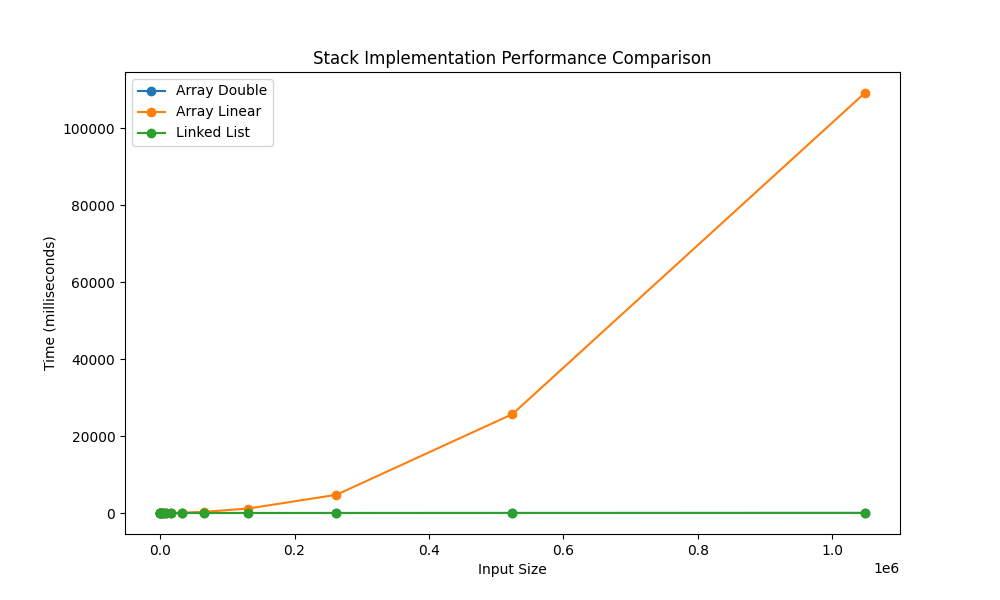
\includegraphics[width=\textwidth]{./images/Figure_1.png}
    \caption{Linear scale axis}
\end{figure}

As we can see from above, the linear capacity increase implementation is by far the slowest, while the other two implementations look like constant time operations. 
One potential discrepancy is that the linear capacity increase implementation seems to have quadratic time, while in theory it should be linear time. 
This could be due to the fact that for larger and larger input sizes, the proportion of push operations that do not require a resize becomes smaller and smaller. 
As a result, the $O(n)$ copying operation is done closer and closer to $n$ times, leading to a quadratic time complexity.
The next graph shows the same data, but with a logarithmic scale on both axes.

\newpage
\begin{figure}[h]
    \centering
    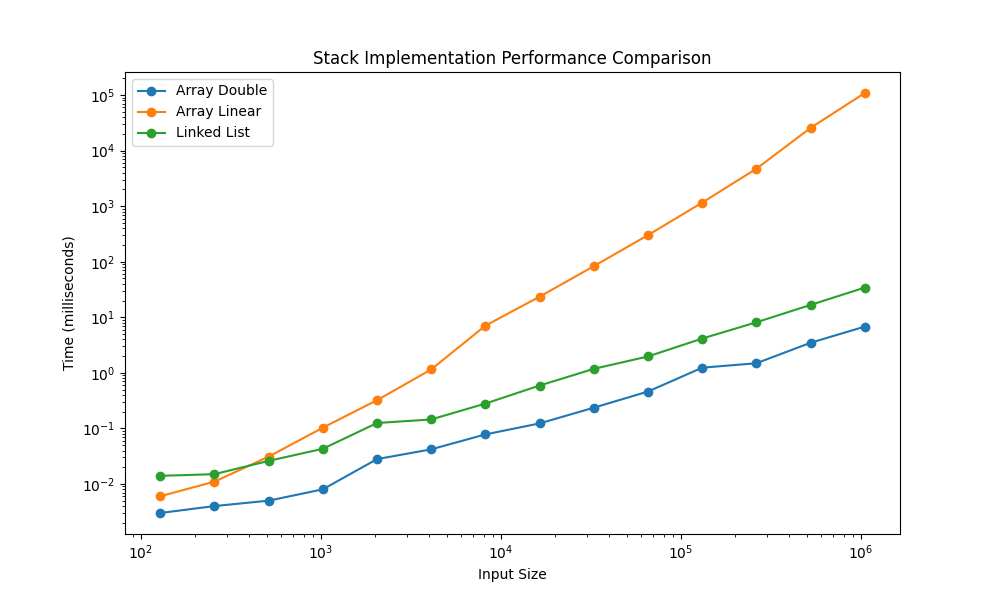
\includegraphics[width=\textwidth]{./images/Figure_2.png}
    \caption{Logarithmic scale axis}
\end{figure}

Now we can see that the doubling capacity implementation and linked list implementation have the same asymptotic behavior, but the doubling capacity implementation is faster by some constant factor. 
This is consistent with our theoretical analysis, since the doubling capacity implementation has an amortized time complexity of $O(1)$, which is the same as the linked list implementation. 
This also makes sense from a code perspective, since the doubling array implementation only has to write a new element for a push, while the linked list implementation has to allocate memory for a new node and change the pointers of the head and the new node. 
We can also see that the linear capacity increase implementation is actually faster than the linked list implementation for small input sizes, but still slower than the doubling capacity implementation. 
This also makes sense, since for small input sizes, this implementation does not have to do too many copying operations, and its typical push operation has less steps than the linked list implementation.

\end{document}
